\documentclass[11pt]{article}
\usepackage{qftnotes}
\usetikzlibrary{decorations.pathmorphing}

\title{Phase 0 $\cdot$ Classical Mechanics --- Lesson 1:\\ Lagrangians and the Euler--Lagrange Equations}
\author{Self-study companion to \emph{Quantum Field Theory for the Gifted Amateur}}
\date{}

\sloppy
\begin{document}
\maketitle

\begin{tcolorbox}[colback=gray!6,colframe=gray!50!black,title={Lesson at a glance},breakable]
\textbf{Prerequisites.} Newton's laws; partial derivatives and the chain rule; integration by parts; basic linear algebra (eigenvalues and eigenvectors of a symmetric matrix); the harmonic oscillator.

\textbf{Time estimate.} About 2--3 hours, plus the exercises (derive everything yourself with the page covered before you read the solution).

\textbf{Learning goals.} By the end you should be able to:
\begin{itemize}[nosep]
  \item set up generalized coordinates and write down $L=T-V$ for a system with constraints;
  \item derive the Euler--Lagrange equations from Hamilton's principle, without looking;
  \item solve the standard examples (oscillator, pendulum, central force, charged particle);
  \item explain why $L$ is not unique, and what a total time derivative does;
  \item find normal modes of a coupled system and say why they are independent oscillators;
  \item write the Lagrangian density of a string, derive the field Euler--Lagrange equation, and recognise the Klein--Gordon Lagrangian.
\end{itemize}
\end{tcolorbox}

\tableofcontents

\section{Why QFT is built on Lagrangians}

Newton's second law, $\vect F = m\vect a$, is a statement about forces on a particle in an inertial frame. It is perfectly good for a block on a ramp, and a poor starting point for a relativistic quantum field. There are three main reasons that QFT is formulated with a \emph{Lagrangian} (more precisely, an \emph{action}) instead.

\begin{enumerate}
  \item \textbf{Manifest Lorentz invariance.} The action $S$ is a single number (a scalar). If we build it from Lorentz scalars, such as $\partial_\mu\phi\,\partial^\mu\phi$ and $\phi^2$, integrated over the invariant volume $\dd^4x$, then Lorentz invariance of the theory is guaranteed by construction. Newton's equation singles out time and does not look relativistic. The equations of motion that follow from a Lorentz-invariant $S$ are automatically Lorentz covariant.
  \item \textbf{Symmetries are easy to read off.} A symmetry of the action implies a conserved quantity (Noether's theorem, Lesson 3). Translation invariance gives momentum, time translation gives energy, rotation gives angular momentum, and an internal phase symmetry gives electric charge. With only equations of motion in hand, such conservation laws are far harder to spot.
  \item \textbf{The path integral.} In the quantum theory the amplitude for a process is a sum over all histories, each weighted by $e^{iS/\hbar}$. The action is thus not merely a clever device for generating equations of motion; it is the object the quantum theory is built from. Stationary action emerges as the classical limit, where the phases of neighbouring paths cancel except near the classical path.
\end{enumerate}

\begin{qftbridge}
Throughout this course we use $\hbar=c=1$ and the metric signature $(+,-,-,-)$, matching Lancaster \& Blundell (L\&B). With $\hbar=1$ the action is dimensionless. In $d=3+1$ dimensions this forces the Lagrangian density to have mass dimension 4. Chapter 1 of L\&B (``Lagrangians'') recaps the formalism on which everything later rests, and chapter 5 (``Continuous systems'') extends it to fields.
\end{qftbridge}

\section{Generalized coordinates and configuration space}

\subsection{Degrees of freedom}

A mechanical system is described at an instant by the information needed to fix its configuration. For $N$ free point particles in three dimensions that is $3N$ Cartesian numbers. Often the system is constrained and fewer numbers suffice, and often a non-Cartesian choice is more natural (an angle for a pendulum).

\begin{definition}[Generalized coordinates]
A set of $n$ independent real numbers $q_1,\dots,q_n$ that uniquely specifies the configuration of the system is called a set of \emph{generalized coordinates}; $n$ is the number of \emph{degrees of freedom}. The space of all possible values of $(q_1,\dots,q_n)$ is the \emph{configuration space}. The $\dot q_i=\dd q_i/\dd t$ are the \emph{generalized velocities}.
\end{definition}

The state of the system at an instant is given by $(q_i,\dot q_i)$ (Newton's second law is second order in time, so positions and velocities are the initial data). The Lagrangian is a function $L(q_1,\dots,q_n,\dot q_1,\dots,\dot q_n,t)$ of this $2n$-dimensional set of variables, plus possibly explicit time.

\subsection{Holonomic constraints}

A \emph{holonomic constraint} is a relation $f(\vect r_1,\dots,\vect r_N,t)=0$ among the Cartesian coordinates (and possibly time). Each independent holonomic constraint removes one degree of freedom. Examples:
\begin{itemize}[nosep]
  \item A plane pendulum: $x^2+y^2=\ell^2$. Two Cartesian coordinates, one constraint, so one degree of freedom, conveniently chosen as the angle $\theta$.
  \item A bead on a rotating hoop: the constraint depends explicitly on time.
  \item A rigid body: all pairwise distances are fixed, leaving six degrees of freedom.
\end{itemize}
Non-holonomic constraints (inequalities, or velocity-dependent relations that cannot be integrated, as for a rolling disc) are outside our scope.

The central practical advantage of the Lagrangian method is that, when we express $T$ and $V$ directly in terms of the independent generalized coordinates, the \emph{forces of constraint} (the tension in the pendulum rod, the normal force of the hoop) never appear. They do no work on virtual displacements consistent with the constraints, and so drop out. We take this (d'Alembert's principle) as given; it is justified in Goldstein ch.~1.

\section{Action, Hamilton's principle, and the Euler--Lagrange equations}

\subsection{The action}

For a system with a single coordinate $q$, the \emph{Lagrangian} is
\begin{equation}
  L(q,\dot q,t)=T-V,
\end{equation}
the kinetic energy minus the potential energy, for the systems we consider here. Given a path $q(t)$ between times $t_1$ and $t_2$, the \emph{action} is
\begin{equation}
  S[q]=\int_{t_1}^{t_2} L\bigl(q(t),\dot q(t),t\bigr)\,\dd t.
\end{equation}
$S$ is a \emph{functional}: it takes a whole function $q(t)$ and returns a number.

\begin{theorem}[Hamilton's principle]
The physical trajectory $q(t)$ with $q(t_1)=q_1$ and $q(t_2)=q_2$ fixed is a stationary point of $S$: $\delta S=0$ under all small variations of the path that keep the endpoints fixed.
\end{theorem}

The word is \emph{stationary}, not ``minimum'': the action is often a minimum for short times, but in general it need only be an extremum or a saddle.

\subsection{Derivation of the Euler--Lagrange equation}

Let $q(t)$ be a path with the given endpoints and let $\eta(t)$ be any smooth function with
\begin{equation}
  \eta(t_1)=\eta(t_2)=0 .
\end{equation}
Consider the one-parameter family of neighbouring paths
\begin{equation}
  q_\varepsilon(t)=q(t)+\varepsilon\,\eta(t).
\end{equation}
All of them have the right endpoints. Now $S[q_\varepsilon]$ is an ordinary function of the single real number $\varepsilon$, and $q$ is stationary exactly when
\begin{equation}
  \left.\diff{}{\varepsilon}S[q_\varepsilon]\right|_{\varepsilon=0}=0\quad\text{for every admissible }\eta .
\end{equation}
Differentiating under the integral sign and using the chain rule, with $\dd q_\varepsilon/\dd\varepsilon=\eta$ and $\dd\dot q_\varepsilon/\dd\varepsilon=\dot\eta$,
\begin{equation}
  \left.\diff{S}{\varepsilon}\right|_0=\int_{t_1}^{t_2}\left(\pdiff{L}{q}\,\eta+\pdiff{L}{\dot q}\,\dot\eta\right)\dd t .
\end{equation}
The second term contains $\dot\eta$, but we want a common factor $\eta$. Integrate by parts:
\begin{equation}
  \int_{t_1}^{t_2}\pdiff{L}{\dot q}\,\dot\eta\,\dd t=\left[\pdiff{L}{\dot q}\,\eta\right]_{t_1}^{t_2}-\int_{t_1}^{t_2}\diff{}{t}\!\left(\pdiff{L}{\dot q}\right)\eta\,\dd t .
\end{equation}
The boundary term vanishes because $\eta(t_1)=\eta(t_2)=0$; \emph{this is the only place the fixed-endpoint condition is used, and it is essential}. Hence
\begin{equation}
  \left.\diff{S}{\varepsilon}\right|_0=\int_{t_1}^{t_2}\left[\pdiff{L}{q}-\diff{}{t}\pdiff{L}{\dot q}\right]\eta(t)\,\dd t=0 .
\end{equation}

\paragraph{Fundamental lemma of the calculus of variations.} If $f(t)$ is continuous on $[t_1,t_2]$ and $\int_{t_1}^{t_2}f\,\eta\,\dd t=0$ for every smooth $\eta$ vanishing at the endpoints, then $f\equiv0$.

\emph{Proof.} Choose $\eta(t)=f(t)(t-t_1)(t_2-t)$, which is admissible when $f$ is smooth (and an approximation argument handles merely continuous $f$). Then $\int f^2(t-t_1)(t_2-t)\,\dd t=0$. The integrand is non-negative and continuous, so it vanishes identically, giving $f(t)=0$ on the open interval and hence everywhere by continuity. $\square$

Applying the lemma with $f=\partial L/\partial q-\frac{\dd}{\dd t}\partial L/\partial\dot q$:

\begin{keyresult}[: Euler--Lagrange]
For $n$ generalized coordinates the stationary-action paths satisfy
\begin{equation}
  \boxed{\;\diff{}{t}\!\left(\pdiff{L}{\dot q_i}\right)-\pdiff{L}{q_i}=0,\qquad i=1,\dots,n.\;}
\end{equation}
\end{keyresult}

\paragraph{Generalization to $n$ coordinates.} Vary each coordinate independently: $q_i\to q_i+\varepsilon\eta_i$ with $\eta_i(t_1)=\eta_i(t_2)=0$. The same steps give $\delta S=\int\sum_i\bigl[\partial L/\partial q_i-\frac{\dd}{\dd t}\partial L/\partial\dot q_i\bigr]\eta_i\,\dd t$. Since the $\eta_i$ are independent (here we need the $q_i$ to be genuinely independent coordinates, i.e.\ the constraints already solved), the lemma is applied to each bracket separately.

\paragraph{Terminology.} The quantity $p_i\equiv\partial L/\partial\dot q_i$ is the \emph{canonical momentum} conjugate to $q_i$, and $\partial L/\partial q_i$ plays the role of a generalized force. The E--L equation then reads $\dot p_i=\partial L/\partial q_i$: a ``Newton's law''. Lesson 2 builds the Hamiltonian formalism from this definition of $p_i$.

\begin{pitfall}
The partial derivatives $\partial L/\partial q$ and $\partial L/\partial\dot q$ treat $q$ and $\dot q$ as \emph{independent variables} of the function $L$. Only \emph{after} taking them do we substitute a path $q(t)$ and evaluate the \emph{total} time derivative $\frac{\dd}{\dd t}$ of $\partial L/\partial\dot q$. That total derivative acts through $q$, $\dot q$ and explicit $t$:
\[
  \diff{}{t}\pdiff{L}{\dot q}=\frac{\partial^2L}{\partial\dot q\,\partial q}\dot q+\frac{\partial^2L}{\partial\dot q^2}\ddot q+\frac{\partial^2L}{\partial\dot q\,\partial t}.
\]
Forgetting the $\dot q$ and $\ddot q$ pieces is a common error. Note also that the E--L equations are second order in time when $\partial^2L/\partial\dot q^2\neq0$.
\end{pitfall}

\section{Worked examples}

\begin{example}[Free particle]
In one dimension, $L=\tfrac12m\dot x^2$. Then $\partial L/\partial\dot x=m\dot x$ and $\partial L/\partial x=0$, so the E--L equation is $\frac{\dd}{\dd t}(m\dot x)=0$: constant velocity, as Newton's first law demands. In three dimensions, $L=\tfrac12m|\dot{\vect r}|^2$ gives three copies of this. Notice that $L$ does not depend on $x$; then $\partial L/\partial x=0$ and $p=m\dot x$ is conserved. This is the simplest instance of the link between a symmetry (translation) and a conservation law, to be generalized in Lesson 3.
\end{example}

\begin{example}[1D harmonic oscillator]
$L=\tfrac12m\dot q^2-\tfrac12kq^2$. Then $\partial L/\partial\dot q=m\dot q$ and $\partial L/\partial q=-kq$. The E--L equation is
\begin{equation}
  m\ddot q=-kq\quad\Longleftrightarrow\quad\ddot q=-\omega^2q,\qquad \omega=\sqrt{k/m},
\end{equation}
with solution $q(t)=A\cos\omega t+B\sin\omega t$. This system, with $L=\tfrac12\dot q^2-\tfrac12\omega^2q^2$ in mass-normalized units, is the building block for everything in the rest of the course.
\end{example}

\begin{example}[Plane pendulum]
A mass $m$ on a massless rigid rod of length $\ell$, with angle $\theta$ measured from the downward vertical. The constraint is already solved by using $\theta$ as the single coordinate. Take the pivot as the origin, with $x=\ell\sin\theta$, $y=-\ell\cos\theta$. Then
\[
 \dot x=\ell\cos\theta\,\dot\theta,\quad \dot y=\ell\sin\theta\,\dot\theta
 \;\Rightarrow\; T=\tfrac12m(\dot x^2+\dot y^2)=\tfrac12m\ell^2\dot\theta^2,
\]
and $V=mgy=-mg\ell\cos\theta$. So
\begin{equation}
  L=\tfrac12m\ell^2\dot\theta^2+mg\ell\cos\theta .
\end{equation}
Now $\partial L/\partial\dot\theta=m\ell^2\dot\theta$ and $\partial L/\partial\theta=-mg\ell\sin\theta$, hence
\begin{equation}
  m\ell^2\ddot\theta=-mg\ell\sin\theta\quad\Longrightarrow\quad\ddot\theta=-\frac g\ell\sin\theta .
\end{equation}
For small angles, $\sin\theta\approx\theta$ and this is a harmonic oscillator with $\omega=\sqrt{g/\ell}$. The rod tension never entered.
\end{example}

\begin{figure}[ht]
\centering
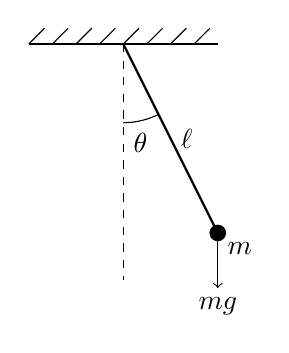
\begin{tikzpicture}[scale=1.0]
  \draw[thick] (-1.2,0) -- (1.2,0);
  \foreach \x in {-1.2,-0.9,...,1.0} \draw (\x,0) -- (\x+0.2,0.2);
  \draw[dashed] (0,0) -- (0,-3);
  \draw[thick] (0,0) -- (1.2,-2.4) node[midway,right] {$\ell$};
  \fill (1.2,-2.4) circle (3pt) node[below right] {$m$};
  \draw (0,-1) arc (-90:-63.4:1);
  \node at (0.22,-1.25) {$\theta$};
  \draw[->] (1.2,-2.4) -- (1.2,-3.1) node[below] {$m\vect g$};
\end{tikzpicture}
\caption{The plane pendulum, with the single generalized coordinate $\theta$.}
\end{figure}

\begin{example}[Central potential in polar coordinates]
A particle of mass $m$ moves in a plane under a potential $V(r)$ depending only on the distance from the origin. Use polar coordinates $(r,\theta)$ with $x=r\cos\theta$, $y=r\sin\theta$. Then $\dot x=\dot r\cos\theta-r\dot\theta\sin\theta$, $\dot y=\dot r\sin\theta+r\dot\theta\cos\theta$, and
\[
  \dot x^2+\dot y^2=\dot r^2+r^2\dot\theta^2 .
\]
Hence
\begin{equation}
  L=\tfrac12m\left(\dot r^2+r^2\dot\theta^2\right)-V(r).
\end{equation}
The two E--L equations are:
\begin{align}
  r:&\quad \diff{}{t}(m\dot r)-mr\dot\theta^2+V'(r)=0\;\Rightarrow\; m\ddot r=mr\dot\theta^2-V'(r),\\
  \theta:&\quad \diff{}{t}\left(mr^2\dot\theta\right)-0=0\;\Rightarrow\; mr^2\dot\theta=\text{const}\equiv \ell_z .
\end{align}
The $\theta$ equation is possible because $\theta$ is \emph{cyclic}: $L$ does not depend on $\theta$ (only on $\dot\theta$). The conserved quantity $\ell_z=mr^2\dot\theta$ is the angular momentum about the origin; the symmetry behind it is rotational invariance of $V(r)$. (Lesson 3 treats this properly.) Eliminating $\dot\theta=\ell_z/(mr^2)$ in the radial equation,
\begin{equation}
  m\ddot r=\frac{\ell_z^2}{mr^3}-V'(r)=-\diff{}{r}\left[V(r)+\frac{\ell_z^2}{2mr^2}\right],
\end{equation}
which is a one-dimensional problem in an \emph{effective potential} with the centrifugal barrier $\ell_z^2/2mr^2$.
\end{example}

\begin{example}[Charged particle in an electromagnetic field]
A particle of charge $q$ and mass $m$ moves in fields $\vect E=-\nabla\phi-\partial_t\vect A$ and $\vect B=\nabla\times\vect A$. The Lagrangian is
\begin{equation}
  L=\tfrac12m\,\dot{\vect x}^2-q\,\phi(\vect x,t)+q\,\dot{\vect x}\cdot\vect A(\vect x,t).
\end{equation}
Here the potential is velocity dependent. Write $\dot{\vect x}\cdot\vect A=\dot x_jA_j$ with a sum over $j$. For the coordinate $x_i$:
\[
 \pdiff{L}{\dot x_i}=m\dot x_i+qA_i,\qquad
 \diff{}{t}\pdiff{L}{\dot x_i}=m\ddot x_i+q\left(\pdiff{A_i}{t}+\dot x_j\,\partial_jA_i\right),
\]
where in the last step $\dd A_i/\dd t=\partial_tA_i+\dot x_j\partial_jA_i$ along the path (a \emph{total} derivative, the pitfall above). And
\[
 \pdiff{L}{x_i}=-q\,\partial_i\phi+q\,\dot x_j\,\partial_iA_j .
\]
The E--L equation is therefore
\begin{equation}
  m\ddot x_i=q\left(-\partial_i\phi-\partial_tA_i\right)+q\,\dot x_j\left(\partial_iA_j-\partial_jA_i\right).
\end{equation}
The first bracket is $qE_i$. For the second, use $\varepsilon_{ijk}\varepsilon_{klm}=\delta_{il}\delta_{jm}-\delta_{im}\delta_{jl}$:
\[
 (\dot{\vect x}\times\vect B)_i=\varepsilon_{ijk}\dot x_j\,\varepsilon_{klm}\partial_lA_m=\dot x_j\left(\partial_iA_j-\partial_jA_i\right).
\]
So
\begin{equation}
  m\ddot{\vect x}=q\left(\vect E+\dot{\vect x}\times\vect B\right),
\end{equation}
the Lorentz force law. Note that the canonical momentum is $p_i=m\dot x_i+qA_i$, \emph{not} $m\dot x_i$; this reappears in Lesson 2.
\end{example}

\begin{qftbridge}
The coupling $-q\phi+q\dot{\vect x}\cdot\vect A$ is the non-relativistic form of $-q\,\dot x^\mu A_\mu$, the seed of the interaction $-j^\mu A_\mu$ in QED (L\&B ch.~14 on gauge fields, and Part IX on QED). The combination $p_i-qA_i$ also reappears as the ``covariant derivative'' $\partial_\mu+iqA_\mu$ that makes a Lagrangian gauge invariant. (See also Exercise~\ref{ex:gauge} below.)
\end{qftbridge}

\section{Non-uniqueness of the Lagrangian}

Different Lagrangians can describe exactly the same physics. The simplest freedom is adding a total time derivative.

\begin{proposition}
Let $F(q_1,\dots,q_n,t)$ be a smooth function and set $L'=L+\dfrac{\dd F}{\dd t}$. Then $L$ and $L'$ have the same Euler--Lagrange equations.
\end{proposition}

\begin{proof}[Proof (via the action)]
$S'[q]=S[q]+F(q(t_2),t_2)-F(q(t_1),t_1)$. The extra term depends only on the endpoints, which are fixed, so $\delta S'=\delta S$. Hence the stationary paths agree.
\end{proof}

\begin{proof}[Proof (direct)]
For one coordinate, $\dfrac{\dd F}{\dd t}=F_q\dot q+F_t$ (subscripts denote partial derivatives; $F$ depends on $q$ and $t$ only). Then
\[
  \pdiff{}{\dot q}\diff{F}{t}=F_q,\qquad \diff{}{t}F_q=F_{qq}\dot q+F_{qt},
\]
\[
  \pdiff{}{q}\diff{F}{t}=F_{qq}\dot q+F_{tq}.
\]
The E--L ``difference'' for the extra term is $F_{qq}\dot q+F_{qt}-F_{qq}\dot q-F_{tq}=0$ by equality of mixed partials. The generalization to $n$ coordinates is identical. $\square$
\end{proof}

\begin{pitfall}
$F$ must not depend on $\dot q$. If it did, $\dd F/\dd t$ would contain $\ddot q$ and the argument above would fail (the boundary term would also involve the unfixed $\dot q$ at the endpoints).
\end{pitfall}

\begin{qftbridge}
Lagrangians that differ by a total derivative have the same equations of motion but can have different Noether charges, because Noether's theorem is derived from how $L$ itself changes under a symmetry. A symmetry transformation may change $L$ only by a total derivative, $\delta L=\dd K/\dd t$, and then the conserved charge picks up a correction from $K$. We will see this in Lesson 3 (and in L\&B ch.~10). For fields, the analogue is $\Lag\to\Lag+\partial_\mu K^\mu$ (Exercise~\ref{ex:fielddiv}); this is why boundary terms in the action can usually be discarded.
\end{qftbridge}

\section{Small oscillations and normal modes}

\subsection{Two coupled masses}

Two identical masses $m$ are attached to two fixed walls by springs of constant $k$, and to each other by a spring of constant $\kappa$. Let $q_1,q_2$ be the displacements from equilibrium along the line.

\begin{figure}[ht]
\centering
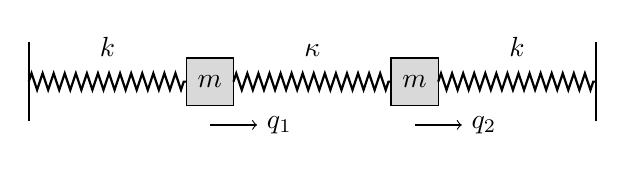
\begin{tikzpicture}
  \draw[thick] (0,-0.5) -- (0,0.5);
  \draw[thick,decorate,decoration={zigzag,segment length=4,amplitude=3}] (0,0) -- (2,0);
  \draw[fill=gray!30] (2,-0.3) rectangle (2.6,0.3); \node at (2.3,0) {$m$};
  \draw[thick,decorate,decoration={zigzag,segment length=4,amplitude=3}] (2.6,0) -- (4.6,0);
  \draw[fill=gray!30] (4.6,-0.3) rectangle (5.2,0.3); \node at (4.9,0) {$m$};
  \draw[thick,decorate,decoration={zigzag,segment length=4,amplitude=3}] (5.2,0) -- (7.2,0);
  \draw[thick] (7.2,-0.5) -- (7.2,0.5);
  \node[above] at (1,0.2) {$k$}; \node[above] at (3.6,0.2) {$\kappa$}; \node[above] at (6.2,0.2) {$k$};
  \draw[->] (2.3,-0.55) -- (2.9,-0.55) node[right] {$q_1$};
  \draw[->] (4.9,-0.55) -- (5.5,-0.55) node[right] {$q_2$};
\end{tikzpicture}
\caption{Two coupled masses between fixed walls.}
\end{figure}

The kinetic energy is $\tfrac12m(\dot q_1^2+\dot q_2^2)$. The potential energy stores $\tfrac12kq_1^2$ in the left spring, $\tfrac12kq_2^2$ in the right spring and $\tfrac12\kappa(q_2-q_1)^2$ in the middle one:
\begin{equation}
  L=\tfrac12m(\dot q_1^2+\dot q_2^2)-\tfrac12k(q_1^2+q_2^2)-\tfrac12\kappa(q_1-q_2)^2 .
\end{equation}
The E--L equations give coupled equations,
\begin{align}
  m\ddot q_1&=-kq_1-\kappa(q_1-q_2),\\
  m\ddot q_2&=-kq_2+\kappa(q_1-q_2).
\end{align}
Because the equations are coupled, neither mass oscillates alone. The symmetry between the masses suggests the combinations
\begin{equation}
  \eta_\pm=\frac{q_1\pm q_2}{\sqrt2},\qquad q_1=\frac{\eta_++\eta_-}{\sqrt2},\quad q_2=\frac{\eta_+-\eta_-}{\sqrt2}.
\end{equation}
This is an orthogonal transformation, so $\dot q_1^2+\dot q_2^2=\dot\eta_+^2+\dot\eta_-^2$ and $q_1^2+q_2^2=\eta_+^2+\eta_-^2$, while $(q_1-q_2)^2=2\eta_-^2$. Therefore
\begin{equation}
  L=\tfrac12m\dot\eta_+^2-\tfrac12k\eta_+^2\;+\;\tfrac12m\dot\eta_-^2-\tfrac12(k+2\kappa)\eta_-^2 .
\end{equation}
The coupling has disappeared: we have \emph{two independent harmonic oscillators} with
\begin{equation}
  \omega_+=\sqrt{\frac km}\ \ (\text{masses move together}),\qquad \omega_-=\sqrt{\frac{k+2\kappa}m}\ \ (\text{masses move oppositely}).
\end{equation}
The middle spring is stretched only in the antisymmetric mode, so only that frequency feels $\kappa$.

\subsection{The general case}

Now let the system have $n$ coordinates and a stable equilibrium at $q_i=q_i^{(0)}$; shift coordinates so it lies at the origin. Expand $T$ and $V$ around it. The kinetic energy is quadratic in velocities, $T=\tfrac12\sum_{ij}M_{ij}(q)\dot q_i\dot q_j$. Since $\dot q$ is already first order in smallness, we may replace $M_{ij}(q)$ by its value at the origin. The potential has $\partial_iV=0$ at equilibrium, and the constant $V(0)$ is irrelevant, so
\begin{equation}
  V\approx\tfrac12\sum_{ij}K_{ij}q_iq_j,\qquad K_{ij}=\left.\frac{\partial^2V}{\partial q_i\partial q_j}\right|_0 .
\end{equation}
Thus, in matrix notation with $\vect q=(q_1,\dots,q_n)^{\mathsf T}$,
\begin{equation}
  L=\tfrac12\dot{\vect q}^{\mathsf T}M\dot{\vect q}-\tfrac12\vect q^{\mathsf T}K\vect q ,
\end{equation}
with $M$ and $K$ real symmetric, $M$ positive definite (kinetic energy is positive), and $K$ positive semi-definite for stability. The E--L equations are
\begin{equation}
  M\ddot{\vect q}=-K\vect q .
\end{equation}

\paragraph{Eigenvalue problem.} Try $\vect q(t)=\vect a\,e^{i\omega t}$ (take the real part at the end). Then
\begin{equation}
  \bigl(K-\omega^2M\bigr)\vect a=0\quad\Longrightarrow\quad\det\bigl(K-\omega^2M\bigr)=0 .
\end{equation}
This is a generalized symmetric eigenvalue problem. Facts that follow from the symmetry and positivity of $M,K$:
\begin{enumerate}[nosep]
  \item The $\omega_r^2$ are real and non-negative. (Take the conjugate transpose with $\vect a^\dagger$: $\omega^2=\vect a^\dagger K\vect a/\vect a^\dagger M\vect a$, a ratio of real non-negative numbers.)
  \item Eigenvectors for distinct eigenvalues are $M$-orthogonal: from $K\vect a_r=\omega_r^2M\vect a_r$ and $K\vect a_s=\omega_s^2M\vect a_s$, we get $\vect a_s^{\mathsf T}K\vect a_r=\omega_r^2\,\vect a_s^{\mathsf T}M\vect a_r$ and, with $r\leftrightarrow s$ and transposing, $\vect a_s^{\mathsf T}K\vect a_r=\omega_s^2\,\vect a_s^{\mathsf T}M\vect a_r$. Subtracting, $(\omega_r^2-\omega_s^2)\,\vect a_s^{\mathsf T}M\vect a_r=0$.
  \item One can therefore choose a basis with $\vect a_s^{\mathsf T}M\vect a_r=\delta_{rs}$ (and then $\vect a_s^{\mathsf T}K\vect a_r=\omega_r^2\delta_{rs}$); degenerate eigenvalues can be orthogonalized by Gram--Schmidt in the $M$ inner product.
\end{enumerate}

\paragraph{Decoupling.} Expand $\vect q(t)=\sum_r\eta_r(t)\,\vect a_r$. Substituting into $L$ and using the orthonormality relations,
\begin{equation}
  L=\sum_{r=1}^n\left(\tfrac12\dot\eta_r^2-\tfrac12\omega_r^2\eta_r^2\right).
\end{equation}
The $\eta_r$ are the \emph{normal coordinates}; each obeys $\ddot\eta_r=-\omega_r^2\eta_r$, an independent harmonic oscillator. Zero eigenvalues $\omega_r=0$ correspond to free (translational) motion.

\begin{keyresult}[: Normal modes]
Any system performing small oscillations about a stable equilibrium is equivalent to a set of \emph{independent harmonic oscillators}, one per normal mode. The frequencies are the roots of $\det(K-\omega^2M)=0$, and the general motion is a superposition of the modes.
\end{keyresult}

\begin{qftbridge}
This is \textbf{the} key idea of the next part of L\&B (Phase 1). A free quantum field has infinitely many degrees of freedom, but its Lagrangian is quadratic, so it decouples into normal modes. Each mode is quantized as a quantum harmonic oscillator, and the excitations of the oscillator for each wavevector are particles. ``Particles are quanta of normal modes of a field''. Make sure you are fluent with this lesson's decoupling procedure and its Fourier-space version (Section~\ref{sec:fields}). The oscillator and occupation-number story is in L\&B chapters 2--4 (simple harmonic oscillators and second quantization); fields as limits of chains appear in chapter 5.
\end{qftbridge}

\section{From particles to fields}\label{sec:fields}

\subsection{A chain of masses and springs}

Take $N$ identical masses $m$ on a line, with equilibrium spacing $a$, joined by springs of constant $K$. Let $q_n(t)$ be the displacement of mass $n$ from its equilibrium position $x_n=na$. Then
\begin{equation}
  L=\sum_n\left[\tfrac12m\dot q_n^2-\tfrac12K\,(q_{n+1}-q_n)^2\right].
\end{equation}

\begin{figure}[ht]
\centering
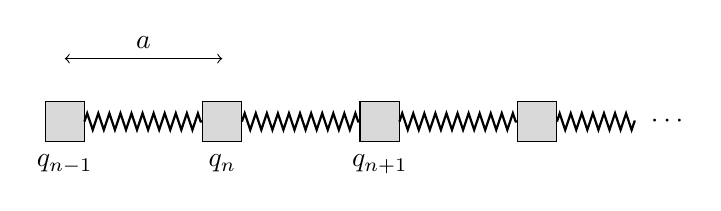
\begin{tikzpicture}[xscale=1.0]
  \foreach \i in {0,1,2,3} {
    \draw[fill=gray!30] (2*\i,-0.25) rectangle (2*\i+0.5,0.25);
  }
  \foreach \i in {0,1,2} {
    \draw[thick,decorate,decoration={zigzag,segment length=4,amplitude=3}] (2*\i+0.5,0) -- (2*\i+2,0);
  }
  \draw[thick,decorate,decoration={zigzag,segment length=4,amplitude=3}] (6.5,0) -- (7.5,0);
  \node at (7.9,0) {$\cdots$};
  \node[below] at (0.25,-0.3) {$q_{n-1}$};
  \node[below] at (2.25,-0.3) {$q_n$};
  \node[below] at (4.25,-0.3) {$q_{n+1}$};
  \draw[<->] (0.25,0.8) -- (2.25,0.8) node[midway,above] {$a$};
\end{tikzpicture}
\caption{A chain of masses and springs; $q_n$ is the displacement of mass $n$ from its site.}
\end{figure}

The E--L equations are $m\ddot q_n=K(q_{n+1}-2q_n+q_{n-1})$.

\subsection{The continuum limit}

Let $a\to0$ with the total length fixed. Introduce the linear mass density $\rho=m/a$ and the tension-like constant $T=Ka$ (the force per unit fractional extension), and let $q_n(t)\to\phi(x,t)$ at $x=na$. Then
\[
  (q_{n+1}-q_n)\approx a\,\partial_x\phi,\qquad \sum_n a\;\to\;\int\dd x .
\]
Rewrite each term of the sum with a factor $a$ pulled out:
\[
  L=\sum_na\left[\tfrac12\frac ma\dot q_n^2-\tfrac12(Ka)\left(\frac{q_{n+1}-q_n}{a}\right)^2\right]\;\longrightarrow\;\int\dd x\left[\tfrac12\rho\left(\pdiff\phi t\right)^2-\tfrac12T\left(\pdiff\phi x\right)^2\right].
\]
The index $n$ labelling the coordinate has become the continuous label $x$: \emph{$x$ is no longer a dynamical variable, just a label}, like the index of $q_n$. The field $\phi(x,t)$ is the dynamical variable, a displacement at each point.

\begin{keyresult}[: Lagrangian density of a string]
The Lagrangian is $L=\int\dd x\,\Lag$ with
\begin{equation}
  \Lag=\tfrac12\rho\,(\partial_t\phi)^2-\tfrac12T\,(\partial_x\phi)^2 ,
\end{equation}
and the action is the spacetime integral $S=\int\dd t\,\dd x\,\Lag$.
\end{keyresult}

\subsection{The field Euler--Lagrange equation}

Generalize to a field $\phi(x^\mu)$ in $d$ spacetime dimensions, with $\Lag=\Lag(\phi,\partial_\mu\phi)$ and action $S=\int\dd^dx\,\Lag$. Vary $\phi\to\phi+\varepsilon\,\delta\phi$, with $\delta\phi=0$ on the boundary of the spacetime region (analogue of the fixed endpoints). Then
\begin{equation}
  \delta S=\int\dd^dx\left[\pdiff\Lag\phi\,\delta\phi+\pdiff\Lag{(\partial_\mu\phi)}\,\partial_\mu(\delta\phi)\right],
\end{equation}
since $\delta(\partial_\mu\phi)=\partial_\mu(\delta\phi)$. Integrate the second term by parts (the divergence theorem in $d$ dimensions):
\[
  \int\dd^dx\,\pdiff\Lag{(\partial_\mu\phi)}\,\partial_\mu(\delta\phi)=\oint\dd\Sigma_\mu\,\pdiff\Lag{(\partial_\mu\phi)}\delta\phi-\int\dd^dx\;\partial_\mu\!\left(\pdiff\Lag{(\partial_\mu\phi)}\right)\delta\phi .
\]
The surface term vanishes since $\delta\phi=0$ there, leaving
\[
  \delta S=\int\dd^dx\left[\pdiff\Lag\phi-\partial_\mu\!\left(\pdiff\Lag{(\partial_\mu\phi)}\right)\right]\delta\phi=0 .
\]
The field version of the fundamental lemma then gives:

\begin{keyresult}[: Field Euler--Lagrange equation]
\begin{equation}
  \boxed{\;\pdiff\Lag\phi-\partial_\mu\!\left(\pdiff\Lag{(\partial_\mu\phi)}\right)=0\;}
\end{equation}
summed over $\mu$. For several fields $\phi_a$ there is one equation for each $a$.
\end{keyresult}

\paragraph{The string.} Treat $(t,x)$ as the coordinates. Then $\partial\Lag/\partial\phi=0$, $\partial\Lag/\partial(\partial_t\phi)=\rho\,\partial_t\phi$ and $\partial\Lag/\partial(\partial_x\phi)=-T\,\partial_x\phi$, so the equation is
\[
  -\partial_t(\rho\,\partial_t\phi)-\partial_x(-T\,\partial_x\phi)=0\;\Longrightarrow\;\rho\,\partial_t^2\phi=T\,\partial_x^2\phi .
\]
This is the wave equation, $\partial_t^2\phi=v^2\partial_x^2\phi$ with $v=\sqrt{T/\rho}$.

\begin{qftbridge}
The field E--L equation and the notion of the Lagrangian density (so that ``position $x$'' becomes a label and the field is the coordinate) are the foundations of L\&B chapter 5, and chapter 7 collects many example Lagrangians. In the relativistic setting the same formula $\partial\Lag/\partial\phi-\partial_\mu(\partial\Lag/\partial(\partial_\mu\phi))=0$ is used for every field in the book.
\end{qftbridge}

\subsection{Preview: the relativistic scalar field}

Now use $\hbar=c=1$, the metric $\eta_{\mu\nu}=\mathrm{diag}(+1,-1,-1,-1)$ and $x^\mu=(t,\vect x)$. A real scalar field in 3+1 dimensions has the Lorentz-invariant Lagrangian density
\begin{equation}
  \Lag=\tfrac12\,\partial_\mu\phi\,\partial^\mu\phi-\tfrac12m^2\phi^2=\tfrac12\dot\phi^2-\tfrac12(\nabla\phi)^2-\tfrac12m^2\phi^2 .
\end{equation}
It has the same structure as the string, with $\rho=T=1$ in three space dimensions, plus a mass term $-\tfrac12m^2\phi^2$ (like an on-site spring; see Exercise~\ref{ex:dispersion}). Compute $\partial\Lag/\partial\phi=-m^2\phi$ and
\[
  \pdiff\Lag{(\partial_\mu\phi)}=\partial^\mu\phi ,
\]
(the factor $\tfrac12$ cancels against the two copies of $\partial\phi$ in $\partial_\nu\phi\,\partial^\nu\phi$). The field E--L equation reads $-m^2\phi-\partial_\mu\partial^\mu\phi=0$, i.e.
\begin{equation}
  \bigl(\partial_\mu\partial^\mu+m^2\bigr)\phi=0,\qquad \partial_\mu\partial^\mu=\partial_t^2-\nabla^2,
\end{equation}
the \emph{Klein--Gordon equation}. For $m=0$ it is the wave equation with speed $1$.

\begin{pitfall}
With signature $(+,-,-,-)$, $\partial_\mu\phi\,\partial^\mu\phi=\dot\phi^2-|\nabla\phi|^2$: the time derivative enters with a plus sign and the spatial derivatives with a minus. The mass term $-\tfrac12m^2\phi^2$ then makes $\Lag=$ ``kinetic $-$ potential'' where the potential is $\tfrac12(\nabla\phi)^2+\tfrac12m^2\phi^2$. Be careful with index positions: $\partial\Lag/\partial(\partial_\mu\phi)=\partial^\mu\phi$ has an \emph{upper} index, so that contracting with the lower-index $\partial_\mu$ gives an invariant. In the opposite signature $(-,+,+,+)$ the Lagrangian is written $-\tfrac12\partial_\mu\phi\partial^\mu\phi-\tfrac12m^2\phi^2$ and the Klein--Gordon operator is $-\partial_t^2+\nabla^2-m^2$; do not mix conventions between books.
\end{pitfall}

\subsection{A field is a collection of oscillators}

Return to the string, clamped at both ends, $\phi(0,t)=\phi(\ell,t)=0$. The functions $\sin(n\pi x/\ell)$, $n=1,2,\dots$, form a complete set on $[0,\ell]$ with
\[
  \int_0^\ell\sin\frac{n\pi x}{\ell}\sin\frac{n'\pi x}{\ell}\,\dd x=\frac\ell2\delta_{nn'},\qquad
  \int_0^\ell\cos\frac{n\pi x}{\ell}\cos\frac{n'\pi x}{\ell}\,\dd x=\frac\ell2\delta_{nn'}\ (n,n'\ge1).
\]
Expand $\phi(x,t)=\sum_{n\ge1}q_n(t)\sin(n\pi x/\ell)$. Then $\partial_x\phi=\sum_n q_n\,(n\pi/\ell)\cos(n\pi x/\ell)$, and
\begin{equation}
  L=\int_0^\ell\Lag\,\dd x=\sum_{n}\left[\frac{\rho\ell}{4}\dot q_n^2-\frac{T\ell}{4}\left(\frac{n\pi}{\ell}\right)^2q_n^2\right].
\end{equation}
The cross terms vanish by orthogonality. This is precisely the sum of independent oscillators, each with effective mass $m_n=\rho\ell/2$ and frequency
\begin{equation}
  \omega_n=\frac{n\pi}{\ell}\sqrt{\frac T\rho}=\frac{n\pi v}{\ell}.
\end{equation}
(From $\tfrac12m_n\dot q_n^2$ one reads off $m_n=\rho\ell/2$, and from $\tfrac12m_n\omega_n^2q_n^2=\tfrac{T\ell}4(n\pi/\ell)^2q_n^2$ one gets $\omega_n^2=(T/\rho)(n\pi/\ell)^2$.)

\begin{keyresult}[: A field is a collection of harmonic oscillators]
A free (quadratic) field decomposes in Fourier modes into infinitely many decoupled harmonic oscillators, one per wavenumber $k$. For the relativistic field, $\omega_k^2=\vect k^2+m^2$.
\end{keyresult}

\begin{qftbridge}
In infinite space, the sine series becomes a Fourier integral: $\phi(\vect x,t)=\int\!\frac{\dd^3k}{(2\pi)^3}\,\tilde\phi_{\vect k}(t)\,e^{i\vect k\cdot\vect x}$, and each $\tilde\phi_{\vect k}$ obeys $\ddot{\tilde\phi}_{\vect k}=-(\vect k^2+m^2)\tilde\phi_{\vect k}$. Quantizing each oscillator is exactly how L\&B builds the free scalar quantum field. Particles with $E_{\vect k}=\sqrt{\vect k^2+m^2}$ are the oscillator quanta (L\&B ch.~6 meets the Klein--Gordon equation, and ch.~11 quantizes the field this way).
\end{qftbridge}

\section{Summary: what to know cold}

\begin{itemize}
  \item Generalized coordinates $q_i$; $L(q,\dot q,t)=T-V$; $S=\int L\,\dd t$.
  \item Hamilton's principle: $\delta S=0$ with fixed endpoints. Derivation: vary, integrate by parts (boundary term dies), fundamental lemma.
  \item E--L: $\frac{\dd}{\dd t}\frac{\partial L}{\partial\dot q_i}-\frac{\partial L}{\partial q_i}=0$. Partial derivatives treat $q,\dot q$ as independent; $\frac{\dd}{\dd t}$ is total.
  \item $p_i=\partial L/\partial\dot q_i$; cyclic coordinate $\Rightarrow$ conserved $p_i$.
  \item $L\to L+\dd F(q,t)/\dd t$ leaves the EOM unchanged.
  \item Charged particle: $L=\tfrac12mv^2-q\phi+q\vect v\cdot\vect A$ gives the Lorentz force.
  \item Small oscillations: $L=\tfrac12\dot{\vect q}^{\mathsf T}M\dot{\vect q}-\tfrac12\vect q^{\mathsf T}K\vect q$; $\det(K-\omega^2M)=0$; normal modes are independent oscillators.
  \item Fields: $L=\int\dd^3x\,\Lag$, $S=\int\dd^4x\,\Lag$; $\partial\Lag/\partial\phi-\partial_\mu\bigl(\partial\Lag/\partial(\partial_\mu\phi)\bigr)=0$.
  \item $\Lag=\tfrac12\partial_\mu\phi\partial^\mu\phi-\tfrac12m^2\phi^2\Rightarrow(\partial_t^2-\nabla^2+m^2)\phi=0$, with $E^2=\vect p^2+m^2$.
  \item A field is a collection of oscillators, one per Fourier mode.
\end{itemize}

\section{Exercises}

\begin{exercise}[Atwood machine]\label{ex:atwood}
Two masses $m_1$ and $m_2$ hang from the ends of a light inextensible string of length $\ell_s$ passing over a frictionless massless pulley. Write the Lagrangian in terms of one generalized coordinate and find the acceleration.
\end{exercise}

\begin{exercise}[Bead on a rotating hoop]\label{ex:hoop}
A bead of mass $m$ slides without friction on a vertical circular hoop of radius $R$ that rotates about its vertical diameter with constant angular velocity $\Omega$. Let $\theta$ be the angle of the bead from the downward vertical. Find $L$ and the equation of motion, find the equilibria, and determine for which $\Omega$ the bottom position $\theta=0$ is stable.
\end{exercise}

\begin{exercise}[Double pendulum]\label{ex:double}
Two plane pendulums are attached in series: mass $m_1$ on a rod of length $\ell_1$ hangs from a fixed pivot, and mass $m_2$ on a rod of length $\ell_2$ hangs from $m_1$. Using the angles $\theta_1,\theta_2$ from the downward vertical, derive $L$ (you need not derive the E--L equations).
\end{exercise}

\begin{exercise}[Total derivative check]\label{ex:totald}
Let $L=\tfrac12m\dot q^2-V(q)$ and $L'=L+\dd F/\dd t$ with $F=\alpha q^2t$, $\alpha$ constant. Compute the E--L equations for $L'$ explicitly and verify that they coincide with those of $L$.
\end{exercise}

\begin{exercise}[Gauge invariance of the charged-particle Lagrangian]\label{ex:gauge}
Show that under $\vect A\to\vect A+\nabla\lambda(\vect x,t)$, $\phi\to\phi-\partial_t\lambda$, the Lagrangian of the charged particle changes by a total time derivative, and that $\vect E$ and $\vect B$ are unchanged.
\end{exercise}

\begin{exercise}[Three-mass chain]\label{ex:three}
Three equal masses $m$ lie on a line between two fixed walls and are joined to each other and to the walls by four identical springs of constant $k$. Find the normal-mode frequencies and mode shapes for longitudinal motion.
\end{exercise}

\begin{exercise}[Dispersion relation of the chain]\label{ex:dispersion}
For the infinite chain with $L=\sum_n[\tfrac12m\dot q_n^2-\tfrac12K(q_{n+1}-q_n)^2]$, find solutions of the form $q_n=e^{i(kna-\omega t)}$ and show that $\omega(k)=2\sqrt{K/m}\,|\sin(ka/2)|$. Show that for $ka\ll1$ this reduces to $\omega=vk$ with $v=\sqrt{T/\rho}$. How would adding a spring of constant $\mu$ from each mass to a fixed point (an ``on-site'' term) change the dispersion relation?
\end{exercise}

\begin{exercise}[A field E--L equation]\label{ex:fieldEL}
Derive the Euler--Lagrange equation for the real scalar field with $\Lag=\tfrac12\partial_\mu\phi\,\partial^\mu\phi-V(\phi)$, and specialize to $V=\tfrac12m^2\phi^2$ and to $V=\tfrac12m^2\phi^2+\tfrac{\lambda}{4!}\phi^4$.
\end{exercise}

\begin{exercise}[Plane waves of Klein--Gordon]\label{ex:KG}
Show that $\phi=e^{-ip\cdot x}$, with $p\cdot x=p_\mu x^\mu=Et-\vect p\cdot\vect x$, solves the Klein--Gordon equation if and only if $E^2=\vect p^2+m^2$. Interpret the two roots $E=\pm\sqrt{\vect p^2+m^2}$ in terms of the general real solution.
\end{exercise}

\begin{exercise}[Total divergences in field theory]\label{ex:fielddiv}
Let $K^\mu(\phi,x)$ be smooth functions of the field and (explicitly) of the spacetime coordinates, and set $\Lag'=\Lag+\partial_\mu K^\mu$. Show that $\Lag'$ and $\Lag$ yield the same field equation. (Here $\partial_\mu K^\mu$ means the total derivative, which includes $\partial_\mu\phi$ via the chain rule.)
\end{exercise}

\section{Solutions}

\begin{solution}{ex:atwood}
Let $x$ be the downward displacement of $m_1$ below the pulley; then $m_2$ is at depth $\ell_s-x$ (neglecting the pulley size), and moves with speed $|\dot x|$. The constraint (fixed string length) leaves one degree of freedom. Then
\[
 T=\tfrac12(m_1+m_2)\dot x^2,\qquad V=-m_1gx-m_2g(\ell_s-x),
\]
so
\[
 L=\tfrac12(m_1+m_2)\dot x^2+(m_1-m_2)gx-m_2g\ell_s .
\]
E--L: $\frac{\dd}{\dd t}\bigl[(m_1+m_2)\dot x\bigr]-(m_1-m_2)g=0$, giving
\[
 \ddot x=\frac{m_1-m_2}{m_1+m_2}\,g .
\]
Checks: $m_1=m_2$ gives zero acceleration; $m_2=0$ gives free fall $g$. The tension (a constraint force) never appeared.
\end{solution}

\begin{solution}{ex:hoop}
Place the origin at the hoop centre. The bead is at cylindrical radius $\rho=R\sin\theta$, height $z=-R\cos\theta$ and azimuth $\Omega t$. Its speed squared is $\dot\rho^2+\rho^2\Omega^2+\dot z^2=R^2\dot\theta^2+R^2\Omega^2\sin^2\theta$. So
\[
 L=\tfrac12mR^2\dot\theta^2+\tfrac12mR^2\Omega^2\sin^2\theta+mgR\cos\theta .
\]
Note that the constraint depends explicitly on $t$, but $L$ in terms of $\theta$ does not, so $\dot\theta\,\partial L/\partial\dot\theta-L$ is conserved, while $T+V$ is not. E--L:
\[
 mR^2\ddot\theta=mR^2\Omega^2\sin\theta\cos\theta-mgR\sin\theta
 \;\Rightarrow\;\ddot\theta=\sin\theta\left(\Omega^2\cos\theta-\frac gR\right).
\]
Equilibria ($\ddot\theta=0$): $\sin\theta=0$ ($\theta=0,\pi$), or $\cos\theta_0=g/(R\Omega^2)$, which exists only if $\Omega^2>g/R$.

Stability of $\theta=0$: linearize with $\sin\theta\approx\theta$, $\cos\theta\approx1$: $\ddot\theta\approx(\Omega^2-g/R)\theta$. This is oscillatory (stable) iff $\Omega^2<g/R$, i.e.\ $\Omega<\sqrt{g/R}$, and exponentially unstable if $\Omega^2>g/R$; at that point the new equilibria at $\theta_0$ appear (a pitchfork bifurcation), and the bead moves out from the bottom. The linearization about $\theta_0$ gives $\ddot\delta=-\Omega^2\sin^2\theta_0\,\delta$, stable.
\end{solution}

\begin{solution}{ex:double}
Positions (origin at the pivot, $y$ upward):
\[
 x_1=\ell_1\sin\theta_1,\quad y_1=-\ell_1\cos\theta_1,\qquad
 x_2=x_1+\ell_2\sin\theta_2,\quad y_2=y_1-\ell_2\cos\theta_2 .
\]
Velocities: $\dot x_1=\ell_1\cos\theta_1\,\dot\theta_1$, $\dot y_1=\ell_1\sin\theta_1\,\dot\theta_1$, so $v_1^2=\ell_1^2\dot\theta_1^2$. For the second mass,
$\dot x_2=\ell_1\cos\theta_1\dot\theta_1+\ell_2\cos\theta_2\dot\theta_2$ and $\dot y_2=\ell_1\sin\theta_1\dot\theta_1+\ell_2\sin\theta_2\dot\theta_2$, so
\[
 v_2^2=\ell_1^2\dot\theta_1^2+\ell_2^2\dot\theta_2^2+2\ell_1\ell_2\dot\theta_1\dot\theta_2\cos(\theta_1-\theta_2).
\]
Then $T=\tfrac12m_1v_1^2+\tfrac12m_2v_2^2$ and $V=m_1gy_1+m_2gy_2=-(m_1+m_2)g\ell_1\cos\theta_1-m_2g\ell_2\cos\theta_2$. Therefore
\[
 L=\tfrac12(m_1+m_2)\ell_1^2\dot\theta_1^2+\tfrac12m_2\ell_2^2\dot\theta_2^2+m_2\ell_1\ell_2\dot\theta_1\dot\theta_2\cos(\theta_1-\theta_2)+(m_1+m_2)g\ell_1\cos\theta_1+m_2g\ell_2\cos\theta_2 .
\]
The kinetic coupling term (not a potential coupling) is what makes the system nonlinear and, for large amplitude, chaotic. Small oscillations: set $\cos(\theta_1-\theta_2)\to1$, $\cos\theta\to1-\theta^2/2$.
\end{solution}

\begin{solution}{ex:totald}
With $\dd F/\dd t=2\alpha qt\,\dot q+\alpha q^2$, we have $L'=\tfrac12m\dot q^2-V(q)+2\alpha qt\,\dot q+\alpha q^2$. Then
\[
 \pdiff{L'}{\dot q}=m\dot q+2\alpha qt,\qquad
 \diff{}{t}\pdiff{L'}{\dot q}=m\ddot q+2\alpha\dot q\,t+2\alpha q,
\]
\[
 \pdiff{L'}{q}=-V'(q)+2\alpha t\,\dot q+2\alpha q .
\]
The E--L equation is $m\ddot q+2\alpha t\dot q+2\alpha q+V'-2\alpha t\dot q-2\alpha q=m\ddot q+V'(q)=0$, identical to that of $L$. Note the canonical momentum did change: $p'=m\dot q+2\alpha qt\neq p$, which is why Lesson 2 will treat canonical momenta as dependent on the choice of $L$.
\end{solution}

\begin{solution}{ex:gauge}
Let $\lambda=\lambda(\vect x,t)$. The new Lagrangian is
\[
 L'=\tfrac12m\dot{\vect x}^2-q(\phi-\partial_t\lambda)+q\dot{\vect x}\cdot(\vect A+\nabla\lambda)=L+q\left(\partial_t\lambda+\dot{\vect x}\cdot\nabla\lambda\right)=L+q\diff\lambda t ,
\]
since along the trajectory $\dd\lambda/\dd t=\partial_t\lambda+\dot x_j\partial_j\lambda$. This is a total derivative of $F=q\lambda(\vect x,t)$, so the equations of motion are unchanged. For the fields: $\vect B'=\nabla\times(\vect A+\nabla\lambda)=\vect B$ because $\nabla\times\nabla\lambda=0$; and $\vect E'=-\nabla(\phi-\partial_t\lambda)-\partial_t(\vect A+\nabla\lambda)=\vect E+\nabla\partial_t\lambda-\partial_t\nabla\lambda=\vect E$.
\end{solution}

\begin{solution}{ex:three}
Let $q_1,q_2,q_3$ be the displacements. The springs have extensions $q_1$, $q_2-q_1$, $q_3-q_2$, $-q_3$, so
\[
 L=\tfrac12m(\dot q_1^2+\dot q_2^2+\dot q_3^2)-\tfrac12k\left[q_1^2+(q_2-q_1)^2+(q_3-q_2)^2+q_3^2\right].
\]
Then $M=m\mathbb 1$ and
\[
 K=k\begin{pmatrix}2&-1&0\\-1&2&-1\\0&-1&2\end{pmatrix}.
\]
Write $\omega^2=(k/m)\lambda$. We need the eigenvalues of the matrix $A$ with $\det(A-\lambda)=(2-\lambda)\bigl[(2-\lambda)^2-1\bigr]-(2-\lambda)=(2-\lambda)\bigl[(2-\lambda)^2-2\bigr]=0$, so $\lambda=2,\ 2\pm\sqrt2$. Hence
\[
 \omega_1^2=(2-\sqrt2)\frac km,\qquad \omega_2^2=2\frac km,\qquad \omega_3^2=(2+\sqrt2)\frac km .
\]
Eigenvectors (unnormalized, from $A\vect a=\lambda\vect a$):
\begin{itemize}[nosep]
 \item $\lambda=2-\sqrt2$: $(1,\sqrt2,1)$. Check row 2: $-1+2\sqrt2-1=2\sqrt2-2=\sqrt2(2-\sqrt2)$. All masses move in phase, the middle one most.
 \item $\lambda=2$: $(1,0,-1)$. The middle mass is at rest; the outer ones oppose each other.
 \item $\lambda=2+\sqrt2$: $(1,-\sqrt2,1)$. Neighbours move oppositely (highest frequency).
\end{itemize}
These are mutually orthogonal (e.g.\ $(1,\sqrt2,1)\cdot(1,-\sqrt2,1)=1-2+1=0$), as expected for a symmetric matrix. They are the first three standing waves $\sin(jn\pi/4)$, $j=1,2,3$, with $\omega_j=2\sqrt{k/m}\sin(j\pi/8)$: indeed $4\sin^2(\pi/8)=2-\sqrt2$, etc.
\end{solution}

\begin{solution}{ex:dispersion}
E--L: $m\ddot q_n=K(q_{n+1}-2q_n+q_{n-1})$. Insert $q_n=e^{i(kna-\omega t)}$:
\[
 -m\omega^2=K\left(e^{ika}+e^{-ika}-2\right)=2K(\cos ka-1)=-4K\sin^2\frac{ka}2 ,
\]
so $\omega=2\sqrt{K/m}\,|\sin(ka/2)|$. For $ka\ll1$, $\omega\approx\sqrt{K/m}\,ka=\sqrt{Ka^2/m}\;k$. With $\rho=m/a$ and $T=Ka$, $T/\rho=Ka^2/m$, so $\omega=vk$ with $v=\sqrt{T/\rho}$ as in the continuum wave equation. The deviation at larger $k$ (the lattice spacing cuts off $k$ at $\pi/a$) is the effect of discreteness.

With an on-site spring $\mu$ the potential gains $\tfrac12\mu q_n^2$, the equation becomes $m\ddot q_n=K(\ldots)-\mu q_n$, and $\omega^2=\mu/m+(4K/m)\sin^2(ka/2)$. In the continuum limit, $\omega^2\approx\mu/m+v^2k^2$: a Klein--Gordon-like dispersion relation, with $\mu/m$ playing the role of $m^2$ (a mass gap).
\end{solution}

\begin{solution}{ex:fieldEL}
Write $\Lag=\tfrac12\eta^{\mu\nu}\partial_\mu\phi\,\partial_\nu\phi-V(\phi)$. Then $\partial\Lag/\partial\phi=-V'(\phi)$. For the derivative, $\partial_\mu\phi$ appears in two places in the quadratic form and $\eta^{\mu\nu}$ is symmetric, so
\[
 \pdiff\Lag{(\partial_\alpha\phi)}=\tfrac12\eta^{\mu\nu}\left(\delta^\alpha_\mu\partial_\nu\phi+\partial_\mu\phi\,\delta^\alpha_\nu\right)=\eta^{\alpha\nu}\partial_\nu\phi=\partial^\alpha\phi .
\]
The field E--L equation $\partial\Lag/\partial\phi-\partial_\alpha(\partial\Lag/\partial(\partial_\alpha\phi))=0$ becomes
\[
 -V'(\phi)-\partial_\alpha\partial^\alpha\phi=0\quad\Longrightarrow\quad\partial_\mu\partial^\mu\phi+V'(\phi)=0,\qquad\text{i.e. }\ \ddot\phi-\nabla^2\phi+V'(\phi)=0 .
\]
For $V=\tfrac12m^2\phi^2$: $V'=m^2\phi$, the Klein--Gordon equation $(\partial_\mu\partial^\mu+m^2)\phi=0$. For $V=\tfrac12m^2\phi^2+\tfrac\lambda{4!}\phi^4$: $V'=m^2\phi+\tfrac\lambda{3!}\phi^3$, so $(\partial_\mu\partial^\mu+m^2)\phi=-\tfrac\lambda{6}\phi^3$, a nonlinear equation (the $\phi^4$ theory).
\end{solution}

\begin{solution}{ex:KG}
For $\phi=e^{-ip\cdot x}=e^{-iEt+i\vect p\cdot\vect x}$: $\partial_t^2\phi=-E^2\phi$ and $\nabla^2\phi=-\vect p^2\phi$. So $(\partial_t^2-\nabla^2+m^2)\phi=(-E^2+\vect p^2+m^2)\phi$, which vanishes iff $E^2=\vect p^2+m^2$. The roots are $E=\pm E_{\vect p}$ with $E_{\vect p}=\sqrt{\vect p^2+m^2}$. For a real field, the general solution is a superposition of $e^{-iE_{\vect p}t+i\vect p\cdot\vect x}$ and its complex conjugate $e^{+iE_{\vect p}t-i\vect p\cdot\vect x}$ (the ``negative-energy'' root is just the complex conjugate, with the sign of $\vect p$ flipped); no independent negative-energy states are involved. Equivalently, for each $\vect p$ the Fourier mode is an oscillator with frequency $\omega_{\vect p}=E_{\vect p}$, and the real general solution is $\sum_{\vect p}\bigl(a_{\vect p}e^{-iE_{\vect p}t+i\vect p\cdot\vect x}+\text{c.c.}\bigr)$. This is the starting point for quantizing the field.
\end{solution}

\begin{solution}{ex:fielddiv}
Let $J\equiv\partial_\mu K^\mu=\dfrac{\partial K^\mu}{\partial\phi}\,\partial_\mu\phi+\dfrac{\partial K^\mu}{\partial x^\mu}\Big|_{\text{expl}}$. Write $K^\mu_\phi=\partial K^\mu/\partial\phi$. Then
\[
 \pdiff J\phi=K^\mu_{\phi\phi}\,\partial_\mu\phi+\partial^{\text{expl}}_\mu K^\mu_\phi,\qquad
 \pdiff J{(\partial_\mu\phi)}=K^\mu_\phi .
\]
The total derivative of the latter is $\partial_\mu K^\mu_\phi=K^\mu_{\phi\phi}\,\partial_\mu\phi+\partial^{\text{expl}}_\mu K^\mu_\phi$, which equals $\partial J/\partial\phi$. So the extra contribution to the E--L expression, $\partial J/\partial\phi-\partial_\mu\bigl(\partial J/\partial(\partial_\mu\phi)\bigr)$, is zero. Alternatively: $\int\dd^dx\,\partial_\mu K^\mu$ is a surface term, which does not change under variations $\delta\phi$ vanishing on the boundary.
\end{solution}

\section*{Suggested further reading}
\addcontentsline{toc}{section}{Suggested further reading}
\begin{itemize}
  \item L.~Susskind and G.~Hrabovsky, \emph{The Theoretical Minimum: What You Need to Know to Start Doing Physics} (Classical Mechanics), Lecture~6 for the principle of least action and Lagrangians (and Lecture~11 for the charged particle). An accessible first pass.
  \item H.~Goldstein, C.~Poole and J.~Safko, \emph{Classical Mechanics}, chapters 1--2: constraints, d'Alembert's principle, Hamilton's principle, and the E--L equations; chapter 6 for small oscillations.
  \item J.~R.~Taylor, \emph{Classical Mechanics}, chapter~7: the Lagrangian approach, with many worked problems and a gentler treatment of the calculus of variations.
  \item D.~Tong, \emph{Classical Dynamics}, Cambridge University lecture notes (freely available online): the Lagrangian formalism and small oscillations.
  \item T.~Lancaster and S.~J.~Blundell, \emph{Quantum Field Theory for the Gifted Amateur}: chapter 1 (Lagrangians), then chapter 5 (continuous systems) and chapter 7 (examples of Lagrangians).
\end{itemize}

\end{document}
